% Copyright (c) 2014,2016 Casper Ti. Vecto
\chapter{系統測試}
於本章將進行功能測試與性能測試,執行功能測試已確認本文所提出之系統的所有功能是否皆順利運行,透過性能測試可知本系統的交易速度在優化前與優化後之間的差異。
	\section{功能測試}
	 	本段主要是描述比特幣的交易監督系統的測試計畫。確認在系統集成前,必須先確認所有的設計元件均可正確的輸出,在此著重於集成系統測試 (Integration Test) 及验收测试 (Acceptance Test)。本章節內容將依據系統需求規格書與系統設計,描述關於集成測試的相關計畫與內容。並希望透過此章節之描述與實踐,達到順利進行測試工作之目的。
	 		\begin{enumerate}
	 			
	 			\item 接受標準:本測試計畫需要滿足下列的測試接受準則: 

	 			\begin{enumerate}
					\item 本系統需要對所有列為必要(Critical、Important、Desirable)之需求作完整測試。
					\item 測試程序需要依照本測試計畫所訂定的程序進行,所有測試結果需要能符合預期測試結果方能接受。
					\item 以測試案例為單位,當測試未通過時,需要進行該單元的測試,其接受的準則與前一項規定相同。 
				\end{enumerate}

				\item 測試環境說明包括所採用的硬件與軟件規格,分別如下:
				\begin{enumerate}
					\item 硬件規格分為系統主機以及週邊設備:
					
					\begin{enumerate}
						\item 系統主機:一台以上主機,每台主機CPU為Intel P4 1.0GHz或以上,256 MB RAM或以上,60G以上硬碟空間。
						\item 周邊設備:一台以上智慧型手機,與用來代表虛擬商品的數個RFID標籤;已可供測試NFC用的智慧型手機包含小米3 WCDMA版,詳細規格於表\ref{mi},Google Nexus 5X,詳細規格於表\ref{5x}。
					
					\end{enumerate}
					\item 軟件規格:關於測試環境所需的軟體規格說明,如下列所示:作業系統:Windows 10、Android 6.0.1/7.1.1

				\end{enumerate}
				\item 測試地點:在銘傳大學桃園校區資工系實驗室,透過Android手機進行的交易模擬實驗,測試環境如圖\ref{fig4}的示意。

%			\end{enumerate}
	 	

	 				\begin{table}[!htbp]
					\centering
					\caption{小米3手機規格}
					\label{mi}
					\begin{tabular}{|l|l|}
					\hline
					系統頻率 & GSM四頻、WCDMA \\ \hline
					作業系統 & Android 4.3 \\ \hline
					處理器 & Qualcomm Snapdragon 800 2.3 GHz四核心 \\ \hline
					記憶體 & 2GB RAM、16GB ROM \\ \hline
					記憶卡 & 不支援 \\ \hline
					顯示螢幕 & 5吋1670萬色IPS(1920×1080 pixels)、441ppi \\ \hline
					相機 & 1300萬畫素(F2.2、28mm)、200萬副鏡頭、1080p \\ \hline
					電池 & 3050 mAh(不可換) \\ \hline
					尺寸 & 144x73.6x8.1mm \\ \hline
					重量 & 145g \\ \hline
					\end{tabular}
					\end{table}

					\begin{table}[!htbp]
					\centering
					\caption{Google Nexus 5X手機規格}
					\label{5x}
					\begin{tabular}{|l|l|}
					\hline
					系統頻率 & GSM四頻、WCDMA \\ \hline
					作業系統 & Android 6.0 \\ \hline
					處理器 & Qualcomm Snapdragon 800 1.8 GHz 六核 \\ \hline
					記憶體 & 2GB RAM、16GB ROM \\ \hline
					記憶卡 & 不支援 \\ \hline
					顯示螢幕 & 5吋1670萬色IPS(1920×1080 pixels)、441ppi \\ \hline
					相機 & 1300萬畫素(F2.2、28mm)、200萬副鏡頭、1080p \\ \hline
					電池 & 2,700 mAh(不可換) \\ \hline
					尺寸 & 147x72.6x7.9mm \\ \hline
					重量 & 136g \\ \hline
					\end{tabular}
					\end{table}

	 		\item 測試時間:

	 			\begin{enumerate}
	 				\item 各子系統之內部元件集成測試 (Module Test)(2017/2/25~2017/6/8)
	 				\item 比特幣的交易監督系統集成測試 (Integration Test) (2017/6/8~2017/6/21)
	 				\item 比特幣的交易監督系統接受度測試 (Acceptance Test) (2017/7/10~2017/7/21)
				\end{enumerate}

			\item 查核點:

				\begin{enumerate}
	 				\item 各子系統之內部元件集成測試 (2017/5/10)
	 				\item 比特幣的交易監督系統集成測試 (2017/7/1)
	 				\item 比特幣的交易監督系統接受度測試 (2017/7/1)
	 			\end{enumerate}

	 		\item 集成测试規劃(Integration Testing):
	 			\begin{figure}[!htbp]
					\centering
					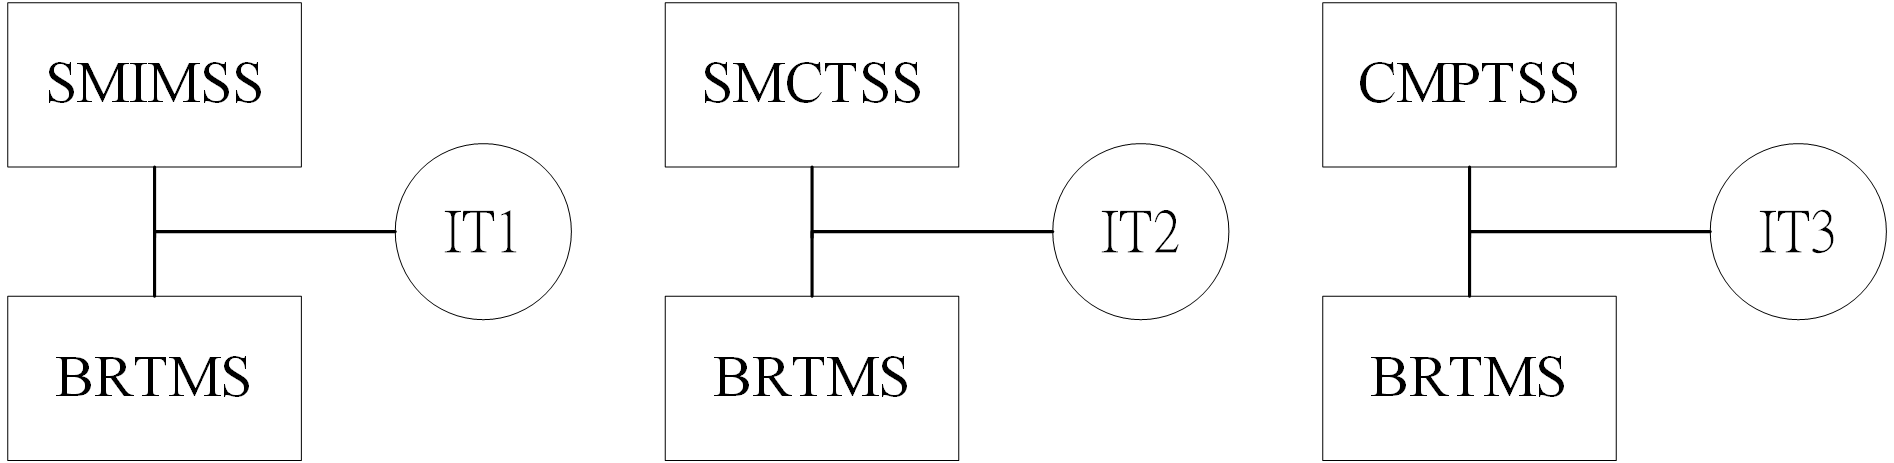
\includegraphics[width = 0.8\textwidth]{IntegrationTesting.png}
					\caption{集成子系統測試}\label{IntegrationTesting}
				\end{figure}
			\item 验收测试規劃(Acceptance Testing,AT):
				本系統須達成以下三組接受用例陳列的所有功能,測試本論文搭設計與搭建的系統功能是否能夠順利運行。測試的角色有兩個,分別為管理員以及使用者,如圖\ref{usecasediagram}為BTMS用例示意圖,預計測試服務器的組態設定、手機的組態設定以及數據庫的組態設定:

					\begin{figure}[!htbp]
						\centering
						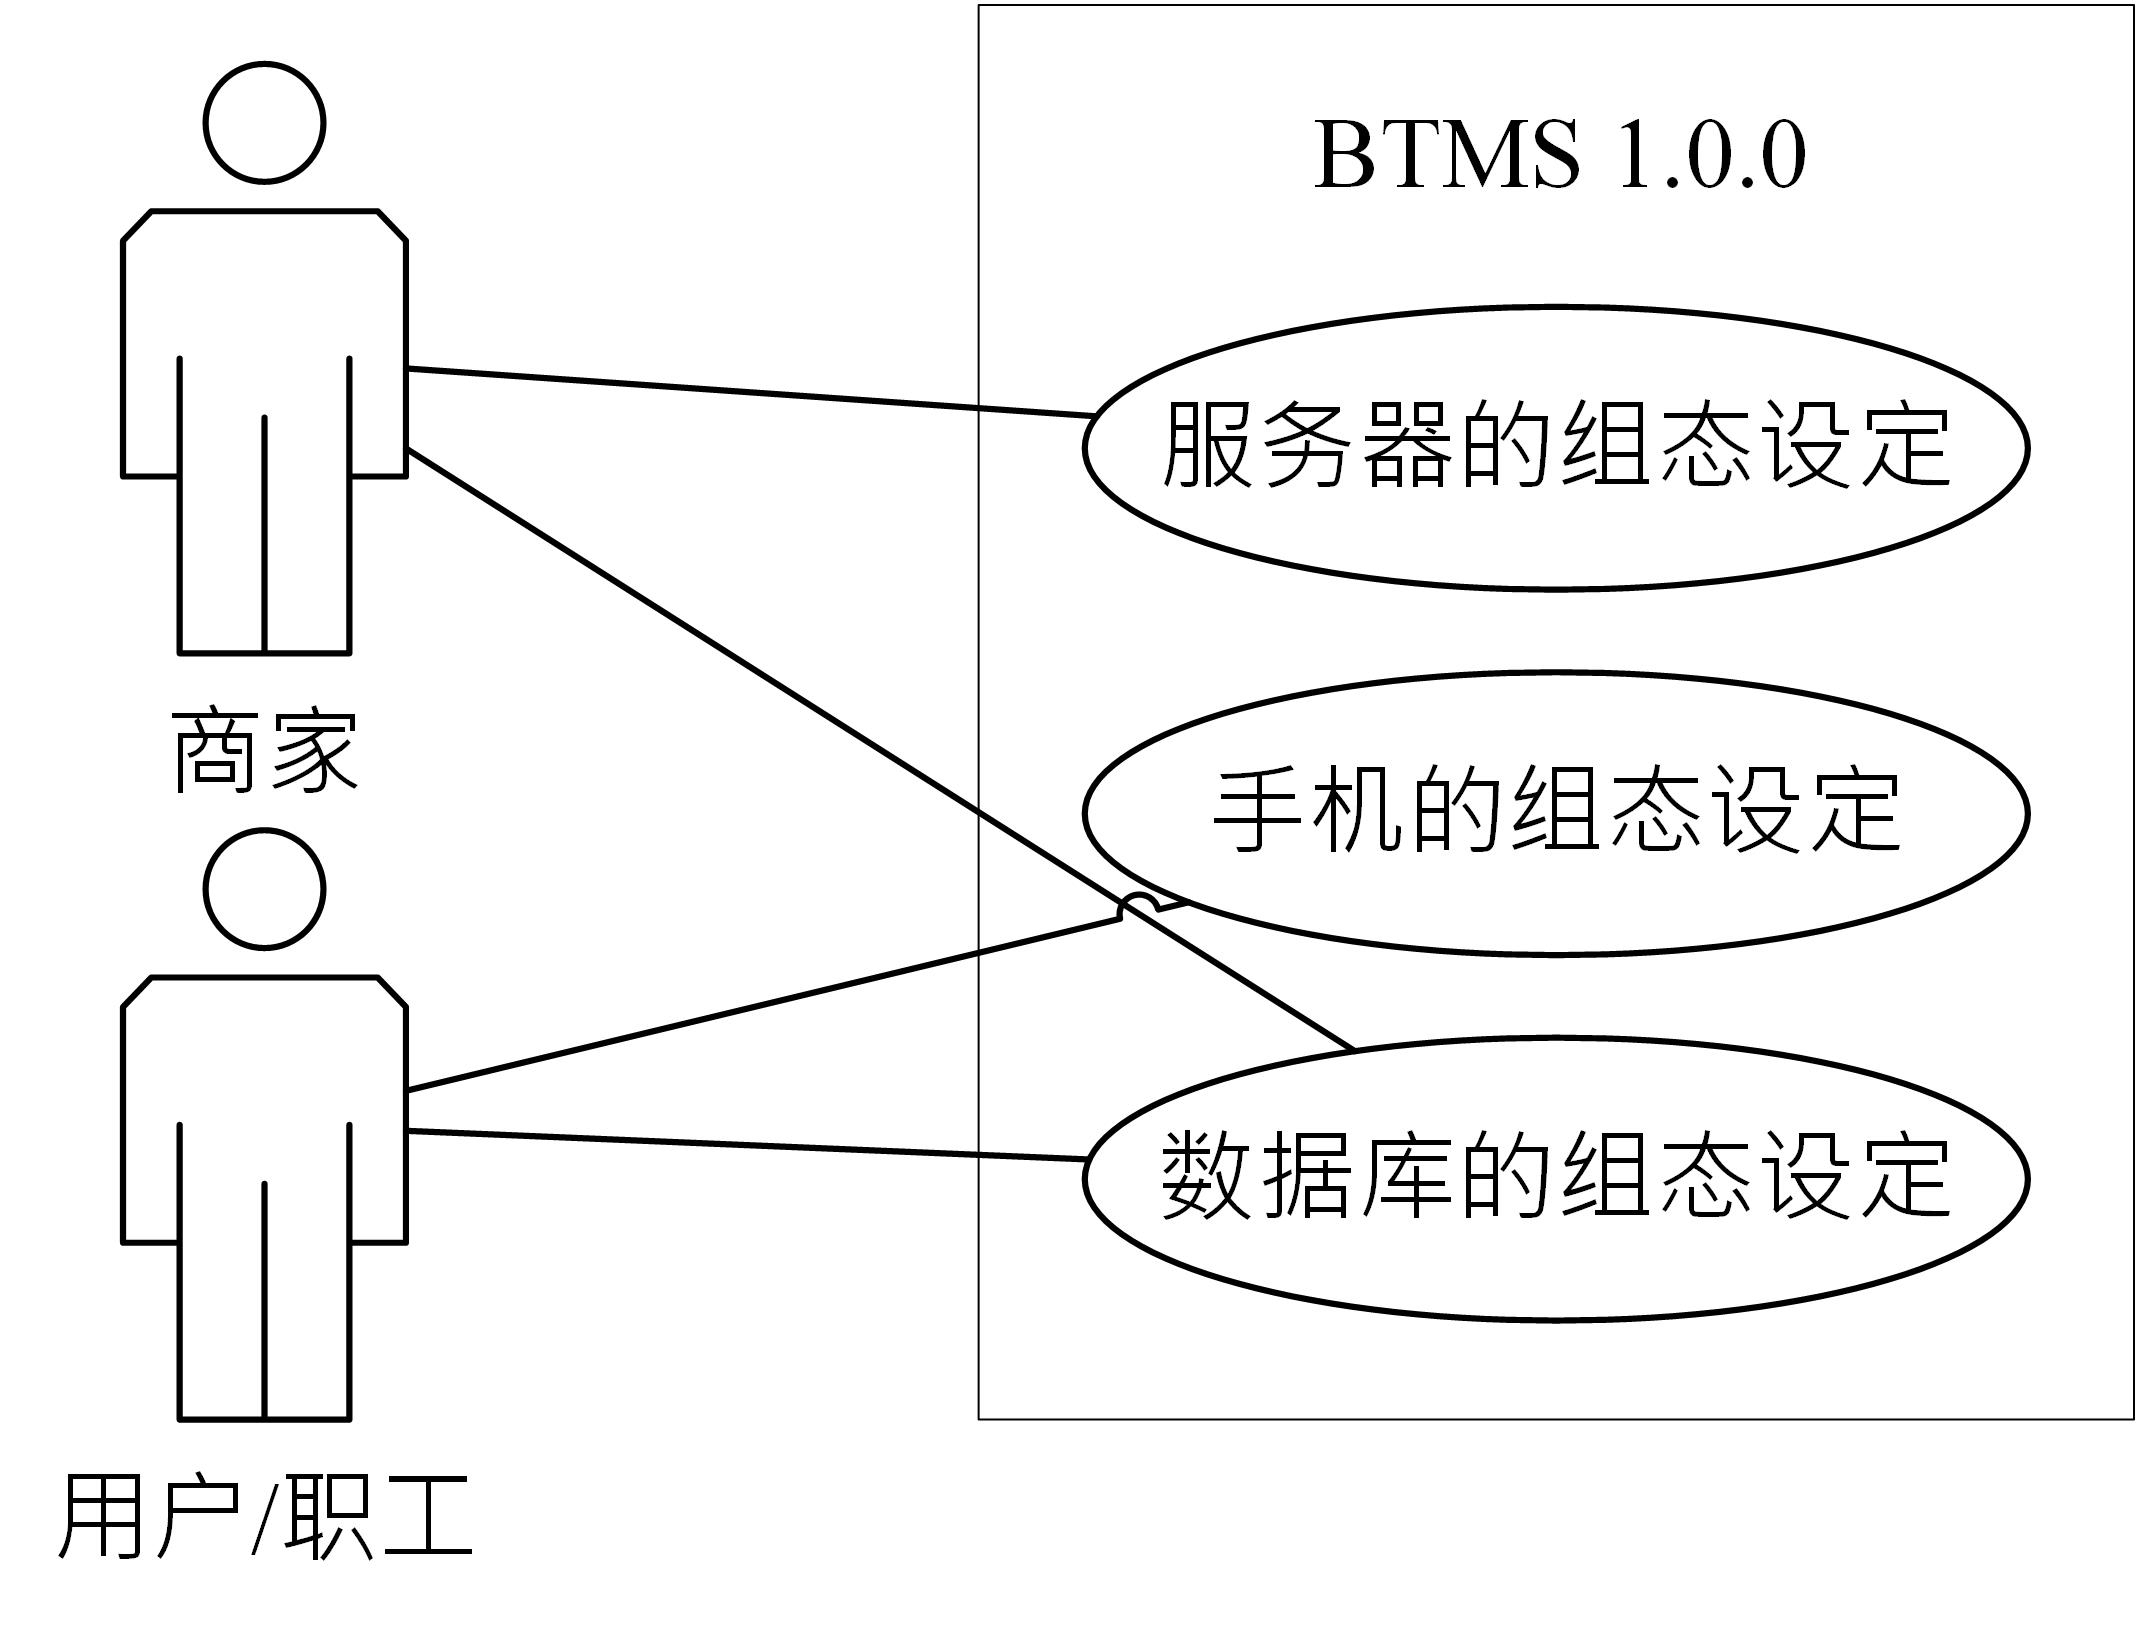
\includegraphics[width = 0.4\textwidth]{usecasediagram.jpg}
						\caption{BTMS使用者用例圖}\label{usecasediagram}
					\end{figure}

				圖\ref{AcceptanceTesting}為三組验收测试的示意圖,對本比特幣的交易監督系統進行測試。
					\begin{figure}[!htbp]
						\centering
						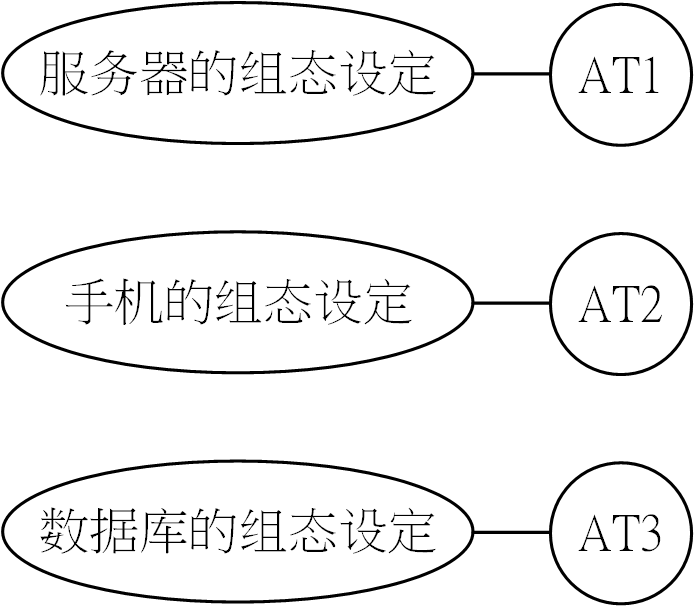
\includegraphics[width = 0.3\textwidth]{AcceptanceTesting.png}
						\caption{验收测试(Acceptance Testing)}\label{AcceptanceTesting}
					\end{figure}

	 		\end{enumerate}			

		\subsection{测试用例}
			\begin{enumerate}

			\item 集成测试(Integration Test)
				\begin{enumerate}

				\item IT1 测试用例:
					表\ref{IT1TestCase}為IT1 测试用例,測試對象為商家端建置與管理商品資訊子系統。目的:驗證〔SMIMSS 1.1.0〕子系統能否正確管理商品資訊。

					\begin{table}[!htbp]
					\centering
					\caption{IT1 测试用例}
					\label{IT1TestCase}
					\begin{tabular}{|l|l|}
					\hline
					用例ID & IT1 \\ \hline
					用例名稱 & 集成SMIMSS至BTMS \\ \hline
					測試目標 & {[}SMIMSS 1.1.0{]}、{[}BTMS 1.0.0{]} \\ \hline
					依賴關係 & SMIMSS-F-001$\sim$ SMIMSS-F-005 \\ \hline
					嚴重程度 & 1(Critical) \\ \hline
					\multirow{5}{*}{用例描述} & 1.     能夠新增店家帳戶 \\ \cline{2-2} 
					 & 2.     能夠新增/修改/刪除店員帳戶 \\ \cline{2-2} 
					 & 3.     能夠新增/刪除/修改商品資訊 \\ \cline{2-2} 
					 & 4.     能夠取得產品資訊 \\ \cline{2-2} 
					 & 5.     能夠接收交易資訊 \\ \hline
					\multirow{5}{*}{預期結果} & 1.     成功新增店家帳戶 \\ \cline{2-2} 
					 & 2.     成功新增/修改/刪除店員帳戶 \\ \cline{2-2} 
					 & 3.     成功新增/修改/刪除商品資訊 \\ \cline{2-2} 
					 & 4.     成功取得產品資訊 \\ \cline{2-2} 
					 & 5.     成功接收交易資訊 \\ \hline
					Cleanup & 無 \\ \hline
					\end{tabular}
					\end{table}


				\item IT2测试用例:
					表\ref{IT2TestCase}為IT2 测试用例麽目標,測試對象為商家端行動收銀與交易明細系統。目的:驗證〔SMCTSS 1.2.0〕子系統是否能夠完成一筆行動支付之交易。

						\begin{table}[!htbp]
						\caption{IT2 测试用例} % title of Table
						\centering % used for centering table
						\label{IT2TestCase} % is used to refer this table in the text
						\begin{tabular}{|l|l|}
						\hline
						用例ID & IT2 \\ \hline
						用例名稱 & 集成SMCTSS至BTMS \\ \hline
						測試目標 & {[}SMCTSS1.2.0{]}、{[}BTMS 1.0.0{]} \\ \hline
						依賴關係 & SMCTSS-F-001$\sim$ SMCTSS-F-007 \\ \hline
						嚴重程度 & 1(Critical) \\ \hline
						\multirow{7}{*}{用例描述} & 1.     能夠登入店員帳戶 \\ \cline{2-2} 
						 & 2.     能夠掃描NFC標籤 \\ \cline{2-2} 
						 & 3.     能夠讀取商品資訊 \\ \cline{2-2} 
						 & 4.     能夠建立交易清單 \\ \cline{2-2} 
						 & 5.     能夠傳送交易資訊 \\ \cline{2-2} 
						 & 6.     能夠認證交易資訊 \\ \cline{2-2} 
						 & 7.     能夠儲存交易明細 \\ \hline
						\multirow{7}{*}{預期結果} & 1.     成功登入店員帳戶 \\ \cline{2-2} 
						 & 2.     成功掃描NFC標籤 \\ \cline{2-2} 
						 & 3.     成功讀取商品資訊 \\ \cline{2-2} 
						 & 4.     成功建立交易清單 \\ \cline{2-2} 
						 & 5.     成功傳送交易資訊 \\ \cline{2-2} 
						 & 6.     成功認證交易資訊 \\ \cline{2-2} 
						 & 7.     成功儲存交易明細 \\ \hline
						Cleanup & 無 \\ \hline
						\end{tabular}
						\end{table}

				\item IT3测试用例:
					表\ref{IT3TestCase}為IT3 测试用例,目標檢測對象為顧客端行動支付與交易明細系統。目的:驗證〔CMPTSS1.3.0〕能正確接收SMCTSS所傳送的交易資料,並以其交易資訊執行以比特幣付款之動作。可以查詢商品資訊,且能夠儲存並且查看使用者過往之交易紀錄。

						\begin{table}[!htbp]
						\caption{IT3 测试用例} % title of Table
						\centering % used for centering table
						\label{IT3TestCase} % is used to refer this table in the text
						\begin{tabular}{|l|l|}
						\hline
						用例ID & IT3 \\ \hline
						用例名稱 & 集成CMPTSS至BTMS \\ \hline
						測試目標 & {[}CMPTSS.1.3.0{]}、{[}BTMS 1.0.0{]} \\ \hline
						依賴關係 & CMPTSS-F-001$\sim$ CMPTSS-F-007 \\ \hline
						嚴重程度 & 1(Critical) \\ \hline
						\multirow{7}{*}{用例描述} & 1.     能夠登入顧客帳號 \\ \cline{2-2} 
						 & 2.     能夠讀取商品資訊 \\ \cline{2-2} 
						 & 3.     能夠接收交易清單 \\ \cline{2-2} 
						 & 4.     能夠認證交易資訊 \\ \cline{2-2} 
						 & 5.     能夠執行行動支付 \\ \cline{2-2} 
						 & 6.     能夠儲存交易明細 \\ \cline{2-2} 
						 & 7.     能夠查看交易紀錄 \\ \hline
						\multirow{7}{*}{預期結果} & 1.     成功登入顧客帳號 \\ \cline{2-2} 
						 & 2.     成功讀取商品資訊 \\ \cline{2-2} 
						 & 3.     成功接收交易清單 \\ \cline{2-2} 
						 & 4.     成功認證交易資訊 \\ \cline{2-2} 
						 & 5.     成功執行行動支付 \\ \cline{2-2} 
						 & 6.     成功儲存交易紀錄 \\ \cline{2-2} 
						 & 7.     成功查看交易紀錄 \\ \hline
						Cleanup & 無 \\ \hline
						\end{tabular}
						\end{table}
				\end{enumerate}

		\item 验收测试用例(Acceptance Testing Cases):
			验收测试用例目的在於測試母系統BTMS、子系統SMIMSS、SMCTSS與CMPTSS是否能夠順利的進行信息傳遞完成交互。

			\begin{enumerate}
				\item AT1 测试用例:
					表\ref{AT1TestCase}所示,目標測試管理人員是否能夠順利使用子系統SMIMSS順利與母系統BTMS交互。目的:驗證使用用例(Use case)1,透過組態檔案的修改對伺服器進行組態設定。

						\begin{table}[!htbp]
						\centering
						\caption{AT1 测试用例}
						\label{AT1TestCase}
						\begin{tabular}{|l|l|l|}
						\hline
						用例ID & \multicolumn{2}{l|}{AT1} \\ \hline
						用例名稱 & \multicolumn{2}{l|}{伺服器的組態設定} \\ \hline
						測試目標 & \multicolumn{2}{l|}{\begin{tabular}[c]{@{}l@{}}{[}SMIMSS 1.1.0{]}\\ {[}BTMS 1.0.0{]}\end{tabular}} \\ \hline
						依賴關係 & \multicolumn{2}{l|}{BTMS-F-001} \\ \hline
						嚴重程度 & \multicolumn{2}{l|}{1} \\ \hline
						\multirow{3}{*}{用例描述} & 使用者操作 & 系統響應 \\ \cline{2-3} 
						 & \begin{tabular}[c]{@{}l@{}}1.管理人員依照環境\\    設定伺服器組態。\end{tabular} &  \\ \cline{2-3} 
						 &  & \begin{tabular}[c]{@{}l@{}}2.伺服器依照管理人\\    員所做的組態設定\\    啟動服務。\end{tabular} \\ \hline
						預期結果 & \multicolumn{2}{l|}{成功啟動伺服器的相關服務。} \\ \hline
						Cleanup & \multicolumn{2}{l|}{無} \\ \hline
						\end{tabular}
						\end{table}

				\item AT2 测试用例:
					如表\ref{AT2TestCase}所示,參與者為使用者。目的:驗證用例(Use case )2 透過組態檔案的修改對手機進行組態設定。
						\begin{table}[!htbp]
						\centering
						\caption{AT2 测试用例}
						\label{AT2TestCase}
						\begin{tabular}{|l|l|l|}
						\hline
						用例ID & \multicolumn{2}{l|}{AT2} \\ \hline
						用例名稱 & \multicolumn{2}{l|}{手機的組態設定} \\ \hline
						測試目標 & \multicolumn{2}{l|}{\begin{tabular}[c]{@{}l@{}}{[}SMCTSS 1.2.0{]}\\ {[}CMPTSS 1.3.0{]}\end{tabular}} \\ \hline
						依賴關係 & \multicolumn{2}{l|}{BTMS-F-002$\sim$ BTMS-F-003} \\ \hline
						嚴重程度 & \multicolumn{2}{l|}{1} \\ \hline
						\multirow{3}{*}{用例描述} & 使用者操作 & 系統響應 \\ \cline{2-3} 
						 & \begin{tabular}[c]{@{}l@{}}1.使用者修改手機組\\    態設定參數。\end{tabular} &  \\ \cline{2-3} 
						 &  & \begin{tabular}[c]{@{}l@{}}2.手機依照使用者在\\    設定檔中所填入的\\    數值運作。\end{tabular} \\ \hline
						預期結果 & \multicolumn{2}{l|}{成功完成手機的組態設定} \\ \hline
						Cleanup & \multicolumn{2}{l|}{無} \\ \hline
						\end{tabular}
						\end{table}

				\item AT3 测试用例:
					如表\ref{AT3TestCase}所示,目的:驗證用例(Use case )3,透過組態檔案的修改對資料庫進行組態設定。

						\begin{table}[!htbp]
						\centering
						\caption{AT3 测试用例}
						\label{AT3TestCase}
						\begin{tabular}{|l|l|l|}
						\hline
						用例ID & \multicolumn{2}{l|}{AT3} \\ \hline
						用例名稱 & \multicolumn{2}{l|}{資料庫的組態設定} \\ \hline
						測試目標 & \multicolumn{2}{l|}{\begin{tabular}[c]{@{}l@{}}{[}SMIMSS 1.1.0{]}\\ {[}SMCTSS 1.2.0{]}\\ {[}CMPTSS 1.3.0{]}\end{tabular}} \\ \hline
						依賴關係 & \multicolumn{2}{l|}{BTMS-F-001$\sim$ BTMS-F-003} \\ \hline
						嚴重程度 & \multicolumn{2}{l|}{1} \\ \hline
						\multirow{5}{*}{用例描述} & 使用者操作 & 系統響應 \\ \cline{2-3} 
						 & \begin{tabular}[c]{@{}l@{}}1.管理者設定資料庫\\    組態。\end{tabular} &  \\ \cline{2-3} 
						 &  & \begin{tabular}[c]{@{}l@{}}2.資料庫依照管理人\\    員所做的組態設定\\    啟動服務。\end{tabular} \\ \cline{2-3} 
						 & \begin{tabular}[c]{@{}l@{}}3.使用者修改資料庫\\    之資料及檔案。\end{tabular} &  \\ \cline{2-3} 
						 &  & \begin{tabular}[c]{@{}l@{}}4.資料庫依照使用者\\    所做的組態設定啟\\    動服務。\end{tabular} \\ \hline
						預期結果 & \multicolumn{2}{l|}{成功設定完成資料庫的相關設定。} \\ \hline
						Cleanup & \multicolumn{2}{l|}{無} \\ \hline
						\end{tabular}
						\end{table}
			\end{enumerate}
		\end{enumerate}

		\subsection{測試結果和分析}
		\begin{enumerate}

			\item 集成測試用例(Integration Testing Cases)
			表\ref{table8}為IT 1、為IT 2、為IT 3的集成子系統測試結果,皆順利運作。

				\begin{table}[!htbp]
				\centering
				\caption{集成子系統測試結果}
				\label{table8}
				\begin{tabular}{|l|l|l|}
				\hline
				测试用例 & 結果 (通過/不通過) & Comment \\ \hline
				\multirow{5}{*}{IT1} & \multirow{5}{*}{通過} & 1.成功新增店家帳戶 \\ \cline{3-3} 
				 &  & 2.成功新增/修改/刪除店員帳戶 \\ \cline{3-3} 
				 &  & 3.成功新增/修改/刪除商品資訊 \\ \cline{3-3} 
				 &  & 4.成功取得產品資訊 \\ \cline{3-3} 
				 &  & 5.成功接收交易資訊 \\ \hline
				\multirow{7}{*}{IT2} & \multirow{7}{*}{通過} & 1.成功登入店員帳戶 \\ \cline{3-3} 
				 &  & 2.成功掃描NFC標籤 \\ \cline{3-3} 
				 &  & 3.成功讀取商品資訊 \\ \cline{3-3} 
				 &  & 4.成功建立交易清單 \\ \cline{3-3} 
				 &  & 5.成功傳送交易資訊 \\ \cline{3-3} 
				 &  & 6.成功認證交易資訊 \\ \cline{3-3} 
				 &  & 7.成功儲存交易明細 \\ \hline
				\multirow{7}{*}{IT3} & \multirow{7}{*}{通過} & 1.成功登入顧客帳號 \\ \cline{3-3} 
				 &  & 2.成功讀取商品資訊 \\ \cline{3-3} 
				 &  & 3.成功接收交易清單 \\ \cline{3-3} 
				 &  & 4.成功認證交易資訊 \\ \cline{3-3} 
				 &  & 5. 成功執行行動支付 \\ \cline{3-3} 
				 &  & 6.成功儲存交易紀錄 \\ \cline{3-3} 
				 &  & 7.成功查看交易紀錄 \\ \hline
				RATE & 90\% & \begin{tabular}[c]{@{}l@{}}BTMS開發透過手機讓商家及顧客\\ 以手機傳送交易資訊,如:商品\\ 名稱、商品金額,商家收款地址。\\ 並且及時將商品資訊更新至伺服器\\ 之資料庫,以便商家控管商品資訊\\ 狀態,同時讓顧客可以享受數位加\\ 密貨幣的方便性。\end{tabular} \\ \hline
				\end{tabular}
				\end{table}

			\item 验收测试用例(Acceptance Testing Cases)
			表\ref{table9}為前節所設計的三種AT 1、AT 2與AT 3的验收测试結果,皆順利運行。
				\begin{table}[!htbp]
				\centering
				\caption{验收测试結果}
				\label{table9}
				\begin{tabular}{|l|l|l|}
				\hline
				测试用例 & 結果(通過/不通過) & Comment \\ \hline
				AT1 & 通過 & 成功啟動伺服器的相關服務。 \\ \hline
				AT2 & 通過 & 成功完成手機的組態設定。 \\ \hline
				AT3 & 通過 & 成功設定完成資料庫的相關設定。 \\ \hline
				Rate & 100\% & \begin{tabular}[c]{@{}l@{}}BTMS可透過組態設定的方式來設\\ 定各個子系統的環境參數。\end{tabular} \\ \hline
				\end{tabular}
				\end{table}
						\begin{table}[!htbp]
						\centering
						\caption{子系統與測試用例關係表}
						\label{table10}
						\begin{tabular}{|l|c|c|c|}
						\hline
						 & \multicolumn{1}{l|}{SMIMSS 1.1.0} & \multicolumn{1}{l|}{SMCTSS 1.2.0} & \multicolumn{1}{l|}{CMPISS 1.3.0} \\ \hline
						IT1 & X &  &  \\ \hline
						IT2 &  & X &  \\ \hline
						IT3 &  &  & X \\ \hline
						AT1 & X &  &  \\ \hline
						AT2 &  & X & X \\ \hline
						AT3 & X & X & X \\ \hline
						\end{tabular}
						\end{table}

						\begin{table}[!htbp]
					\centering
					\caption{需求與集成測試用例的關係表}
					\label{table11}
					\begin{tabular}{|l|c|c|c|}
					\hline
					 & \multicolumn{1}{l|}{IT1} & \multicolumn{1}{l|}{IT2} & \multicolumn{1}{l|}{IT3} \\ \hline
					BTMS-F-001 & X &  &  \\ \hline
					BTMS-F-002 &  & X &  \\ \hline
					BTMS-F-003 &  &  & X \\ \hline
					SMIMSS-F-001 & X &  &  \\ \hline
					SMIMSS-F-002 & X &  &  \\ \hline
					SMIMSS-F-003 & X &  &  \\ \hline
					SMIMSS-F-004 & X &  &  \\ \hline
					SMIMSS-F-005 & X &  &  \\ \hline
					SMCTSS-F-001 &  & X &  \\ \hline
					SMCTSS-F-002 &  & X &  \\ \hline
					SMCTSS-F-003 &  & X &  \\ \hline
					SMCTSS-F-004 &  & X &  \\ \hline
					SMCTSS-F-005 &  & X &  \\ \hline
					SMCTSS-F-006 &  & X &  \\ \hline
					SMCTSS-F-007 &  & X &  \\ \hline
					CMPTSS-F-001 &  &  & X \\ \hline
					CMPTSS-F-002 &  &  & X \\ \hline
					CMPTSS-F-003 & \multicolumn{1}{l|}{} & \multicolumn{1}{l|}{} & X \\ \hline
					CMPTSS-F-004 & \multicolumn{1}{l|}{} & \multicolumn{1}{l|}{} & X \\ \hline
					CMPTSS-F-005 & \multicolumn{1}{l|}{} & \multicolumn{1}{l|}{} & X \\ \hline
					CMPTSS-F-006 & \multicolumn{1}{l|}{} & \multicolumn{1}{l|}{} & X \\ \hline
					CMPTSS-F-007 & \multicolumn{1}{l|}{} & \multicolumn{1}{l|}{} & X \\ \hline
					\end{tabular}
					\end{table}


					\begin{table}[!htbp]
					\centering
					\caption{需求與验收测试案例的關係表}
					\label{table12}
					\begin{tabular}{|l|c|c|c|}
					\hline
					 & \multicolumn{1}{l|}{AT1} & \multicolumn{1}{l|}{AT2} & \multicolumn{1}{l|}{AT3} \\ \hline
					BTMS-F-001 & X &  & X \\ \hline
					BTMS-F-002 &  & X & X \\ \hline
					BTMS-F-003 &  & X & X \\ \hline
					\end{tabular}
					\end{table}


			\item 可追蹤性(Traceability)

						

			\begin{enumerate}
				\item 子系統與測試用例:表\ref{table10}為測試組IT 1、IT 2、IT 3、AT 1、AT 2、AT 3與子系統SMIMSS、SMCTSS、CMPISS的關係表。
				\item 需求與測試用例:表\ref{table11}為本系統需求與集成測試用例的關係表,表\ref{table12}為需求與验收测试案例的關係表。
				\end{enumerate}
		\end{enumerate}







	\section{性能測試}


		\begin{figure}[!htbp]
			\centering
			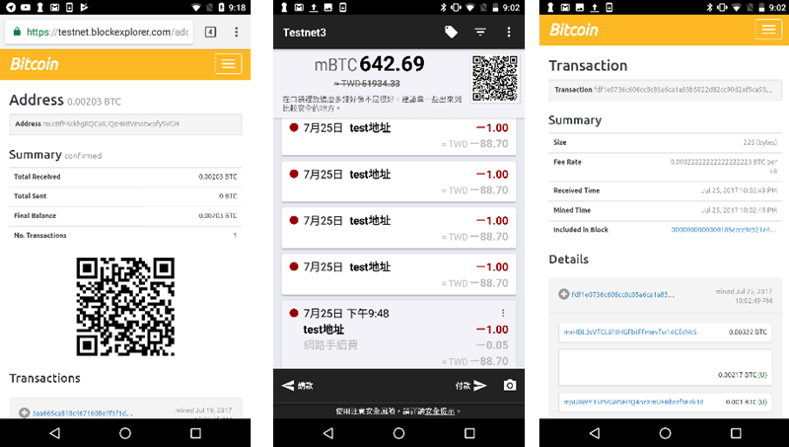
\includegraphics[width = 0.8\textwidth]{fig9.png}
			\caption{使用區塊鏈瀏覽器驗證存儲在比特幣區塊鏈中的交易過程}\label{fig9}
		\end{figure}


		根據比特幣點對點架構,儘管顧客和商家之間的交易細節已經快速存儲到雲數據庫,但官方確認交易與當前比特幣區塊鏈的交易通常需要更長的時間,因為需要確保確認的數量在交易廣播比特幣點對點網絡並存儲到緩存池後,是否存在雙重支付。本文設計了比特幣的交易监督系统以及引用多重簽章算法重新設計的比特幣的實時交易监督系统,以下將分別針對有無採用多重簽章算法的性能測試。


		\subsection{系统性能測試}
		為了驗證本文提出的BTMS不會通過使用比特幣等加密貨幣影響交易完成時間,於2017年7月25日、2017年9月6日以及2018年3月21日,在Testnet實驗中連續記錄了20筆交易信息,每1秒發出一筆交易,分別歷時20分鐘。

		\begin{enumerate}
			\item 初始測試(2017年7月25日):
			首先,使用區塊鏈檢視器(Blockchain Explorer)\supercite{Blockchainexplorer:Ananalyticalprocessandinvestigationenvironmentforbitcoin},如\ref{fig9}的快照所示,透過使用Testnet依序進行20筆比特幣交易,如圖\ref{fig9}的中間快照所示,最後20筆交易完成時間全部記錄在區塊鏈檢視器。實驗結果顯示,實驗中的所有交易都在3秒鐘左右(平均2.97秒,標準差小於1秒)發送到比特幣網絡緩存池,平均交易完成時間在比特幣區塊鏈中確認為522.33秒(小於9分鐘),標準差大約為339秒。

			\item 第一次測試(2017年9月6日):表\ref{1general}為第一次實驗數據,該次的比特幣交易發起廣播至比特幣交易緩存持的時間平均為1.918秒,標準差為0.55586秒。但為了預防雙重支付攻擊需要等待平均654.8秒(小於11分鐘,標準差346.63秒)的時間。

				\begin{table}[!htbp]
				\centering
				\caption{第一次Testnet 執行實驗之數據分析(2017年9月6日)}
				\label{1general}
				\begin{tabular}{|l|l|l|l|}
				\hline
				 & 進入緩存池時間(秒) & 進入區塊鏈時間(秒) & 完成交易時間(秒) \\ \hline
				平均 & 1.918 & 654.8 & 654.8 \\ \hline
				樣本標準差 & 0.55586 & 346.63 & 346.63 \\ \hline
				95\%信賴區間 & 1.69$\sim$2.15 & 511.72$\sim$797.88 & 511.72$\sim$797.88 \\ \hline
				99\%信賴區間 & 1.61$\sim$2.23 & 460.9$\sim$848.7 & 460.9$\sim$848.7 \\ \hline
				\end{tabular}
				\end{table}

			\item 第二次測試(2018年3月21日):表\ref{2general}為第二次測試的實驗原始數據,表\ref{2general-1}為將數據進行分析後的結果可以看出,平均進入緩存持的時間為1.12秒,進入區塊鏈的時間為287.12秒,因為並未採用多重簽章算法,所以交易完成時間以287.12秒計算。
				\begin{table}[!htbp]
				\centering
				\caption{第二次Testnet 執行實驗數據(2018年3月21日)}
				\label{2general}
				\begin{tabular}{|c|c|c|c|c|c|}
				\hline
				\begin{tabular}[c]{@{}c@{}}交易\\ 次數\end{tabular} & 付款時間 & \begin{tabular}[c]{@{}c@{}}進入緩存池\\ 所花時間(秒)\end{tabular} & \begin{tabular}[c]{@{}c@{}}進入緩存池\\ 時間點\end{tabular} & \begin{tabular}[c]{@{}c@{}}寫入區塊鏈\\ 所花時間(秒)\end{tabular} & \begin{tabular}[c]{@{}c@{}}寫入區塊\\ 時間點\end{tabular} \\ \hline
				1 & 0:00:00 & 3 & 0:00:03 & 136 & 0:02:16 \\ \hline
				2 & 0:01:00 & 1 & 0:01:01 & 76 & 0:02:16 \\ \hline
				3 & 0:02:04 & 3 & 0:02:07 & 12 & 0:02:16 \\ \hline
				4 & 0:03:00 & 1 & 0:03:01 & 438 & 0:10:18 \\ \hline
				5 & 0:04:00 & 1 & 0:04:01 & 378 & 0:10:18 \\ \hline
				6 & 0:05:00 & 1 & 0:05:01 & 318 & 0:10:18 \\ \hline
				7 & 0:06:00 & 2 & 0:06:02 & 258 & 0:10:18 \\ \hline
				8 & 0:07:00 & 1 & 0:07:01 & 198 & 0:10:18 \\ \hline
				9 & 0:08:00 & 1 & 0:08:01 & 138 & 0:10:18 \\ \hline
				10 & 0:09:00 & 1 & 0:09:01 & 78 & 0:10:18 \\ \hline
				11 & 0:10:00 & 1 & 0:10:01 & 18 & 0:10:18 \\ \hline
				12 & 0:11:00 & 2 & 0:11:02 & 810 & 0:24:30 \\ \hline
				13 & 0:12:00 & 1 & 0:12:01 & 750 & 0:24:30 \\ \hline
				14 & 0:13:00 & 1 & 0:13:01 & 690 & 0:24:30 \\ \hline
				15 & 0:14:00 & 1 & 0:14:01 & 630 & 0:24:30 \\ \hline
				16 & 0:15:00 & 1 & 0:15:01 & 570 & 0:24:30 \\ \hline
				17 & 0:16:00 & 2 & 0:16:02 & 510 & 0:24:30 \\ \hline
				18 & 0:17:00 & 2 & 0:17:02 & 450 & 0:24:30 \\ \hline
				19 & 0:18:00 & 1 & 0:18:01 & 390 & 0:24:30 \\ \hline
				20 & 0:19:00 & 1 & 0:19:01 & 330 & 0:24:30 \\ \hline
				\end{tabular}
				\end{table}

				\begin{table}[!htbp]
				\centering
				\caption{第二次以Testnet 執行實驗數據分析(2018年3月21日)}
				\label{2general-1}
				\begin{tabular}{|l|l|l|l|}
				\hline
				 & 進入緩存池時間(秒) & 進入區塊鏈時間(秒) & 完成交易時間(秒) \\ \hline
				平均 & 1.12 & 287.12 & 287.12 \\ \hline
				樣本標準差 & 0.68 & 246.59 & 246.59 \\ \hline
				95\%信賴區間 & 0.84$\sim$1.4 & 185.33$\sim$388.91 & 185.33$\sim$388.91 \\ \hline
				99\%信賴區間 & 0.74$\sim$1.5 & 149.18$\sim$425.06 & 149.18$\sim$425.06 \\ \hline
				\end{tabular}
				\end{table}


		\end{enumerate}

			在未引用多重簽章算法的監督系統中,第一次與第二次的測試相比並無太大的差異,交易完成時間與比特幣區塊生成所需時間相同,平均時間皆為十分鐘。根據比特幣Testnet上的初步實驗結果顯示,本文提出的BTMS可以快速有效地執行比特幣的交易监督系统。

			%

		\subsection{實時系统性能測試}
		本主要介紹比特幣測試幣於Government Green Address錢包進行交易的效能實驗與結果分析,包含該實驗的目的、方法及結果分析。實驗的目的是要確認的系統在商家端進行行動支付時能快速、精準且高效率的進行交易,並瞭解使用一般Testnet錢包與Government Green Address錢包作為交易媒介的確認交易時間的差距。表\ref{0test}為2017年7月25日初步的採用多重簽章算法的測試數據,數據顯示交易存儲到區塊鏈的平均時間為10分鐘,但Government Green Address採用的多重簽章算法,可以有效拒絕雙重花費的交易發起,因此可將交易的有效時間,從交易進入區塊鏈的時間,重新訂定為交易進入比特幣交易緩存持的時間。

		\begin{table}[!htbp]
			\centering
			\caption{初步的Government Green Address實驗測試數據 (2017年7月25日)}
			\label{0test}
			\begin{tabular}{|l|l|l|l|l|}
			\hline
			\multicolumn{1}{|c|}{付款時間} & \multicolumn{1}{c|}{\begin{tabular}[c]{@{}c@{}}進入緩存池\\ 所花時間(秒)\end{tabular}} & \multicolumn{1}{c|}{\begin{tabular}[c]{@{}c@{}}進入緩存池\\ 時間點\end{tabular}} & \multicolumn{1}{c|}{入塊時間} & \multicolumn{1}{c|}{\begin{tabular}[c]{@{}c@{}}寫入區塊\\ 費時間\end{tabular}} \\ \hline
			06:36:25 & 02:14 & 06:36:27.14 & 06:52:00 & 16:25 \\ \hline
			06:38:25 & 1.075 & 06:38:26.075 & 06:52:00 & 14:25 \\ \hline
			06:40:25 & 1.722 & 06:40:26.722 & 06:52:00 & 12:25 \\ \hline
			06:42:25 & 2.953 & 06:42:27.953 & 06:52:00 & 10:25 \\ \hline
			06:44:25 & 1.511 & 06:44:26.511 & 06:52:00 & 08:25 \\ \hline
			06:46:25 & 2.269 & 06:46:27.269 & 06:52:00 & 06:25 \\ \hline
			06:48:25 & 1.831 & 06:48:26.831 & 06:52:00 & 04:25 \\ \hline
			06:50:25 & 1.227 & 06:50:26.227 & 06:52:00 & 02:25 \\ \hline
			06:52:25 & 2.026 & 06:52:27.026 & 07:12:01 & 20:24 \\ \hline
			06:54:25 & 1.257 & 06:54:26.257 & 07:12:01 & 18:24 \\ \hline
			06:56:25 & 1.511 & 06:56:26.511 & 07:12:01 & 16:24 \\ \hline
			06:58:25 & 2.815 & 06:58:27.815 & 07:12:01 & 14:24 \\ \hline
			07:00:26 & 1.544 & 07:00:27.544 & 07:12:01 & 12:25 \\ \hline
			07:02:25 & 1.767 & 07:02:26.767 & 07:12:01 & 10:24 \\ \hline
			07:04:25 & 1.52 & 07:04:26.52 & 07:12:01 & 08:24 \\ \hline
			07:06:25 & 1.953 & 07:06:26.953 & 07:12:01 & 06:24 \\ \hline
			\end{tabular}
			\end{table}


		本次的實驗分為兩部份,分別是透過比特幣 Testnet錢包以及使用本論文所採用的Government Green Address比特幣錢包上執行20次付款,皆以相同地址收款,交易金額都設定為0.00001BTC,實驗時間為2017年9月6日與2018年2月6日,每隔一分鐘執行一次付款的動作,總共歷時20分鐘。兩款錢包同時發起交易,並透過區塊鏈檢視器進行記錄時間,最後再比較使用一般比特幣錢包及Government Green Address錢包兩者之間的差距。

		\begin{enumerate}
			\item 第一次測試(2017年9月6日):表\ref{1green}為第一次測試實驗的數據分析結果,平均進入交易緩存池的時間為2.11秒,真正寫入區塊鏈的時間為654.24秒,採用多重簽章算法,這些交易不存在雙重支付的問題,因此完成時間記為2.11秒。

			\begin{table}[!htbp]
				\centering
				\caption{第一次以Government Green Address執行實驗之數據分析(2017年9月6日)}
				\label{1green}
				\begin{tabular}{|l|l|l|l|}
				\hline
				 & 進入緩存池時間(秒) & 進入區塊鏈時間(秒) & 完成交易時間(秒) \\ \hline
				平均 & 2.11 & 654.24 & 2.11 \\ \hline
				樣本標準差 & 0.65 & 346.9 & 0.65 \\ \hline
				95\%信賴區間 & 1.84$\sim$2.38 & 511.05$\sim$797.43 & 1.84$\sim$2.38 \\ \hline
				99\%信賴區間 & 1.75$\sim$2.47 & 460.19$\sim$848.29 & 1.75$\sim$2.47 \\ \hline
				\end{tabular}
				\end{table}

			\item 第二次測試(2018年3月21日):表\ref{2green}為第二次以Government Green Address執行實驗數據,表\ref{2green-1}為基於第二次測試的數據分析結果,進入緩存池的平均時間為1.55秒,進入區塊鏈的平均時間為431.4秒,因為採用多重簽章算法將完成交易時間以1.55秒計算。

		\end{enumerate}
			\begin{table}[!htbp]
				\centering
				\caption{第二次以Government Green Address執行實驗數據(2018年3月21日)}
				\label{2green}
				\begin{tabular}{|c|c|c|c|c|c|}
				\hline
				\begin{tabular}[c]{@{}c@{}}交易\\ 次數\end{tabular} & 付款時間 & \begin{tabular}[c]{@{}c@{}}進入緩存池\\ 所花時間(秒)\end{tabular} & \begin{tabular}[c]{@{}c@{}}進入緩存池\\ 時間點\end{tabular} & \begin{tabular}[c]{@{}c@{}}寫入區塊鏈\\ 所花時間(秒)\end{tabular} & \begin{tabular}[c]{@{}c@{}}寫入區塊\\ 時間點\end{tabular} \\ \hline
				1 & 0:00:01 & 2 & 0:00:03 & 619 & 0:10:18 \\ \hline
				2 & 0:01:00 & 1 & 0:01:01 & 559 & 0:10:18 \\ \hline
				3 & 0:02:02 & 2 & 0:02:04 & 496 & 0:10:18 \\ \hline
				4 & 0:03:00 & 1 & 0:03:01 & 438 & 0:10:18 \\ \hline
				5 & 0:04:00 & 1 & 0:04:01 & 378 & 0:10:18 \\ \hline
				6 & 0:05:00 & 2 & 0:05:02 & 318 & 0:10:18 \\ \hline
				7 & 0:06:00 & 1 & 0:06:01 & 258 & 0:10:18 \\ \hline
				8 & 0:07:00 & 1 & 0:07:01 & 198 & 0:10:18 \\ \hline
				9 & 0:08:00 & 2 & 0:08:02 & 138 & 0:10:18 \\ \hline
				10 & 0:09:00 & 2 & 0:09:02 & 78 & 0:10:18 \\ \hline
				11 & 0:10:00 & 1 & 0:10:01 & 18 & 0:10:18 \\ \hline
				12 & 0:11:00 & 2 & 0:11:02 & 810 & 0:24:30 \\ \hline
				13 & 0:12:00 & 2 & 0:12:02 & 750 & 0:24:30 \\ \hline
				14 & 0:13:00 & 1 & 0:13:01 & 690 & 0:24:30 \\ \hline
				15 & 0:14:00 & 2 & 0:14:02 & 630 & 0:24:30 \\ \hline
				16 & 0:15:00 & 1 & 0:15:01 & 570 & 0:24:30 \\ \hline
				17 & 0:16:00 & 2 & 0:16:02 & 510 & 0:24:30 \\ \hline
				18 & 0:17:00 & 2 & 0:17:02 & 450 & 0:24:30 \\ \hline
				19 & 0:18:00 & 1 & 0:18:01 & 390 & 0:24:30 \\ \hline
				20 & 0:19:00 & 2 & 0:19:02 & 330 & 0:24:30 \\ \hline
				\end{tabular}
				\end{table}

			\begin{table}[!htbp]
				\centering
				\caption{第二次以Government Green Address執行實驗之數據分析(2018年3月21日)}
				\label{2green-1}
				\begin{tabular}{|l|l|l|l|}
				\hline
				 & 進入緩存池時間(秒) & 進入區塊鏈時間(秒) & 完成交易時間(秒) \\ \hline
				平均 & 1.55 & 431.4 & 1.55 \\ \hline
				樣本標準差 & 0.51 & 220.84 & 0.51 \\ \hline
				95\%信賴區間 & 1.34$\sim$1.76 & 340.24$\sim$522.56 & 1.34$\sim$1.76 \\ \hline
				99\%信賴區間 & 1.26$\sim$1.84 & 307.86$\sim$554.94 & 1.26$\sim$1.84 \\ \hline
				\end{tabular}
				\end{table}

				

				
				

	%			\begin{figure}[!htbp]
	%				\centering
	%				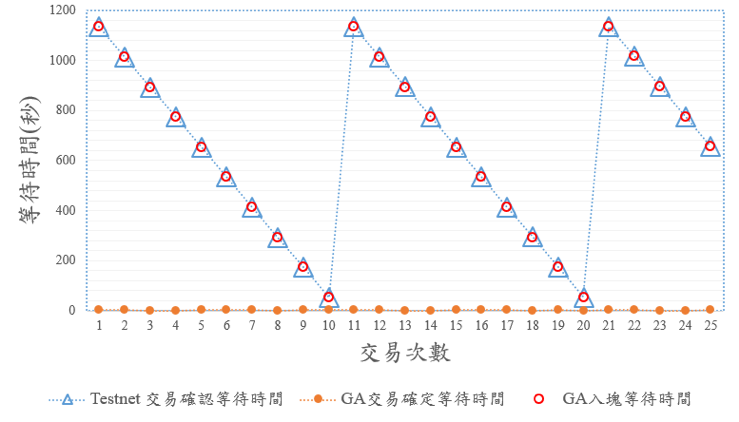
\includegraphics[width = 0.7\textwidth]{fig12.png}
	%				\caption{fig12}\label{fig12}
	%

%				\end{figure}

	本次實驗分別記錄以Testnet錢包及Government Green Address錢包執行20次交易的進入緩存池等待時間和寫入區塊等待時間。若以Testnet錢包交易,必須等到交易寫入才能保證此筆交易不會被礦工遺棄,也才算真的完成這筆交易;但若以Government Green Address錢包發起交易就大不相同,當交易進入緩存池,即使遇到交易被礦工遺棄的情況,Government Green Address機構節點也會重新發起此筆交易,保證讓交易寫入區塊,所以只要進入緩存池就可以視為交易完成,透過兩者錢包的交易數據,本文分析兩種錢包交易的時間數據。

	\begin{table}[!htbp]
	\centering
	\caption{原始系統與實時系統比較表}
	\label{generalvsga}
	\begin{tabular}{|c|c|}
	\hline
	 & 完成交易時間(秒) \\ \hline
	原始系统交易平均時間 & 287.12 \\ \hline
	實時系统交易平均時間 & 1.55 \\ \hline
	\end{tabular}
	\end{table}

	透過本次的實驗可以發現雖然以兩種錢包交易進入區塊的等待時間完全相同,但因為Government Green Address錢包的特性,只要進入緩存池就算完成交易確認,因此Government Green Address錢包的完成交易確認的時間遠遠快於一般Testnet。相信以此⽅式作為主要⽀付管道,可以省去顧客在現金⽀付時掏零錢、算錢及找零等繁瑣的動作及時間,以此達成提升⽇常⽣活中的便利性與安全性。



		